
\subsection{Summary of the parameters used for resources extrapolation}
A table with the parameters that are used for the resources extrapolation is provided. These parameters are in three categories,  (i) computing parameters such as CPU usage per event and event size, and (ii) computing model parameters such as number of replicas and number of (re)processings needed, (iii) physics parameters such LHC luminosity, trigger rate and number of events to be simulated 
The 
\subsection{The method used}
A short description of the python model used and how parameters dependencies can be studied independently. A derivative of the resources vs parameter should be  calculated, so the parameters with the largest impact on resources are listed

%\subsection{Possible scenarios}
%Different scenarios are identified. From a minimal %scenario where we do data reconstruction and little %simulation to the "ideal" scenario where we do all %simulation we need. The dependency on fast vs G4 %simulation is expected to be quite important 

\subsection{Projections for the Three Scenario}
Provide CPU, disk and tape needed projections in the Conservative, Baseline, and Aggressive scenarios. Provide resources extrapolations for 10\%/year and 20\%/year increases.

All the plots are ATLAS internal,  the parameters are still being discussed.    
Plots on the impact on physics performances should also be added, either here or in a different section





\begin{figure}[h]
    \centering
    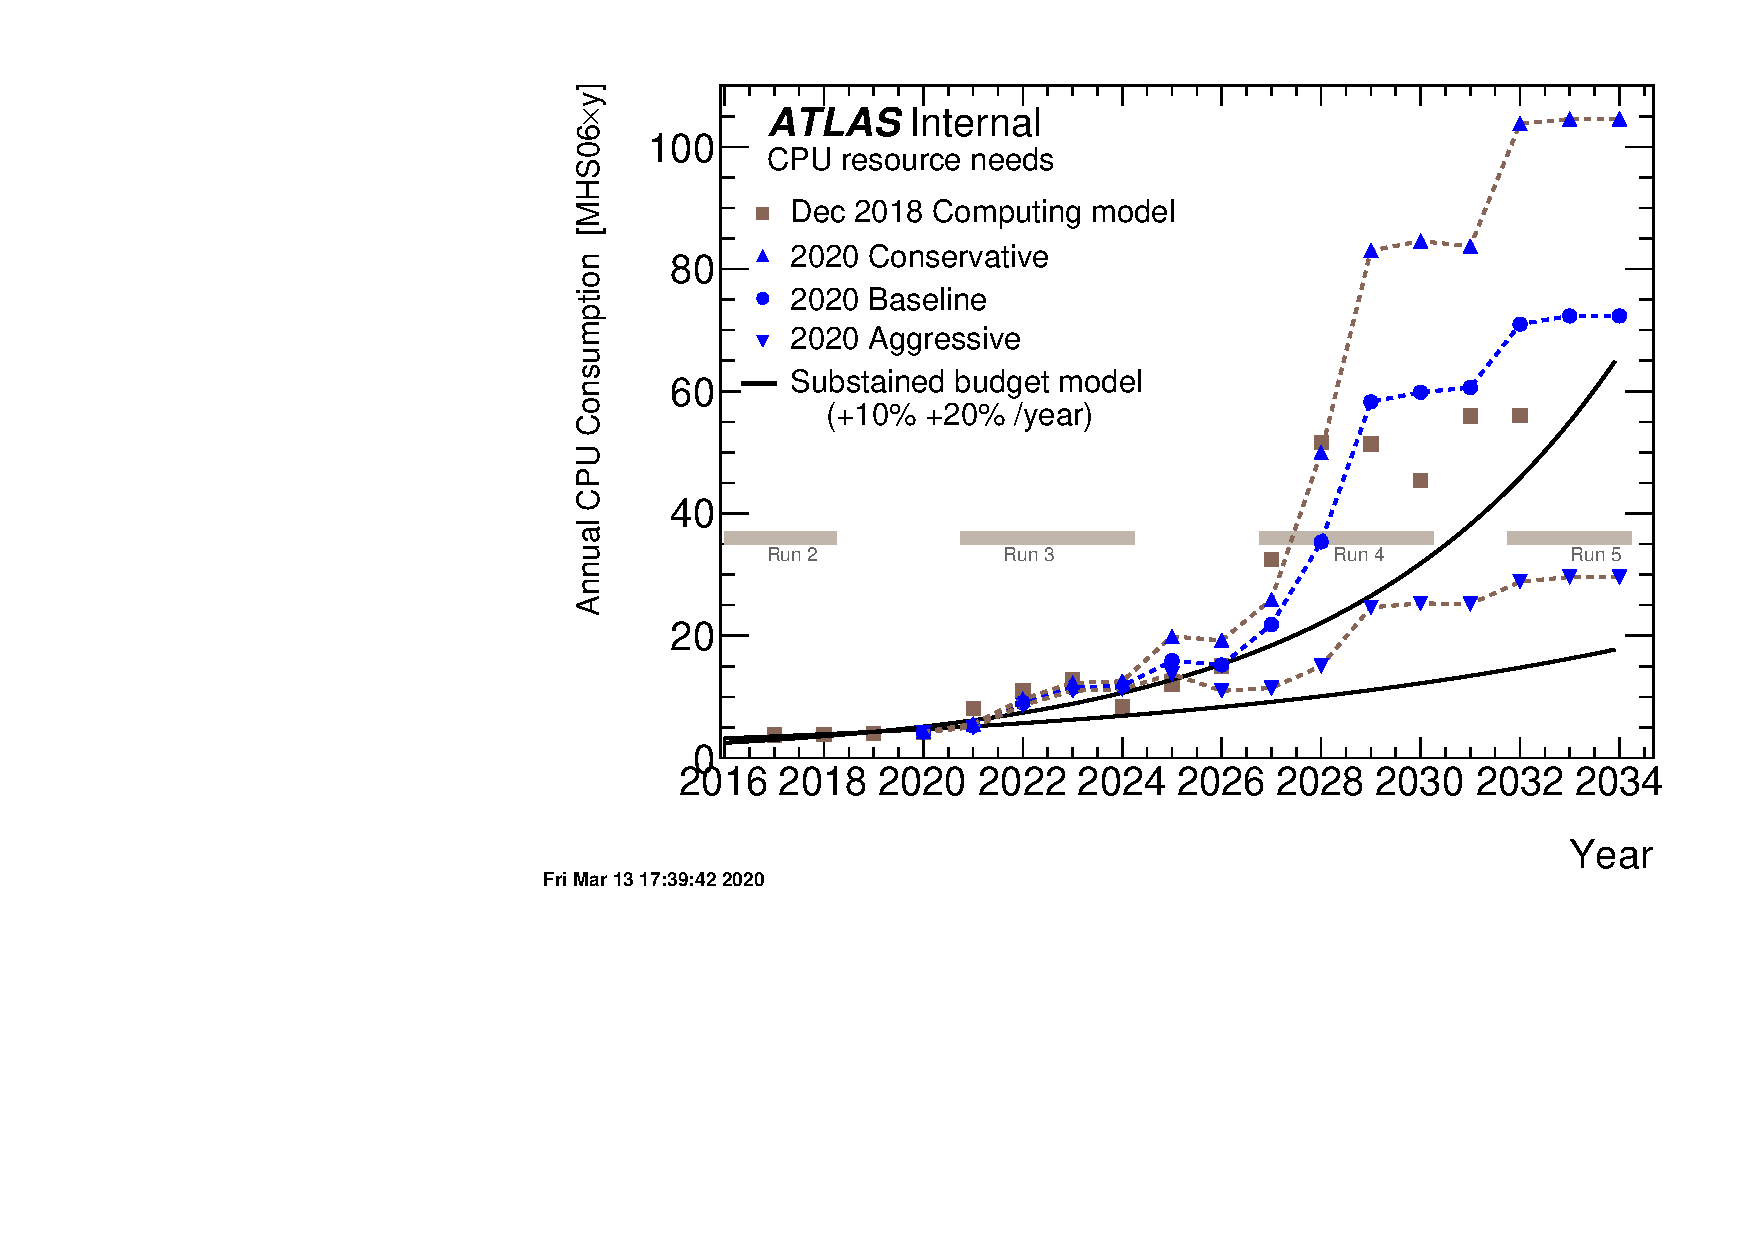
\includegraphics[width=0.80\textwidth]{figures/cpuHLLHC_comparison_2020_InputData_11March.pdf}
   \caption{ Estimated total CPU resources  needed  for the years 2020 to  2034.    }  
    \label{fig:cpu}
\end{figure}





\begin{figure}[h]
    \centering
    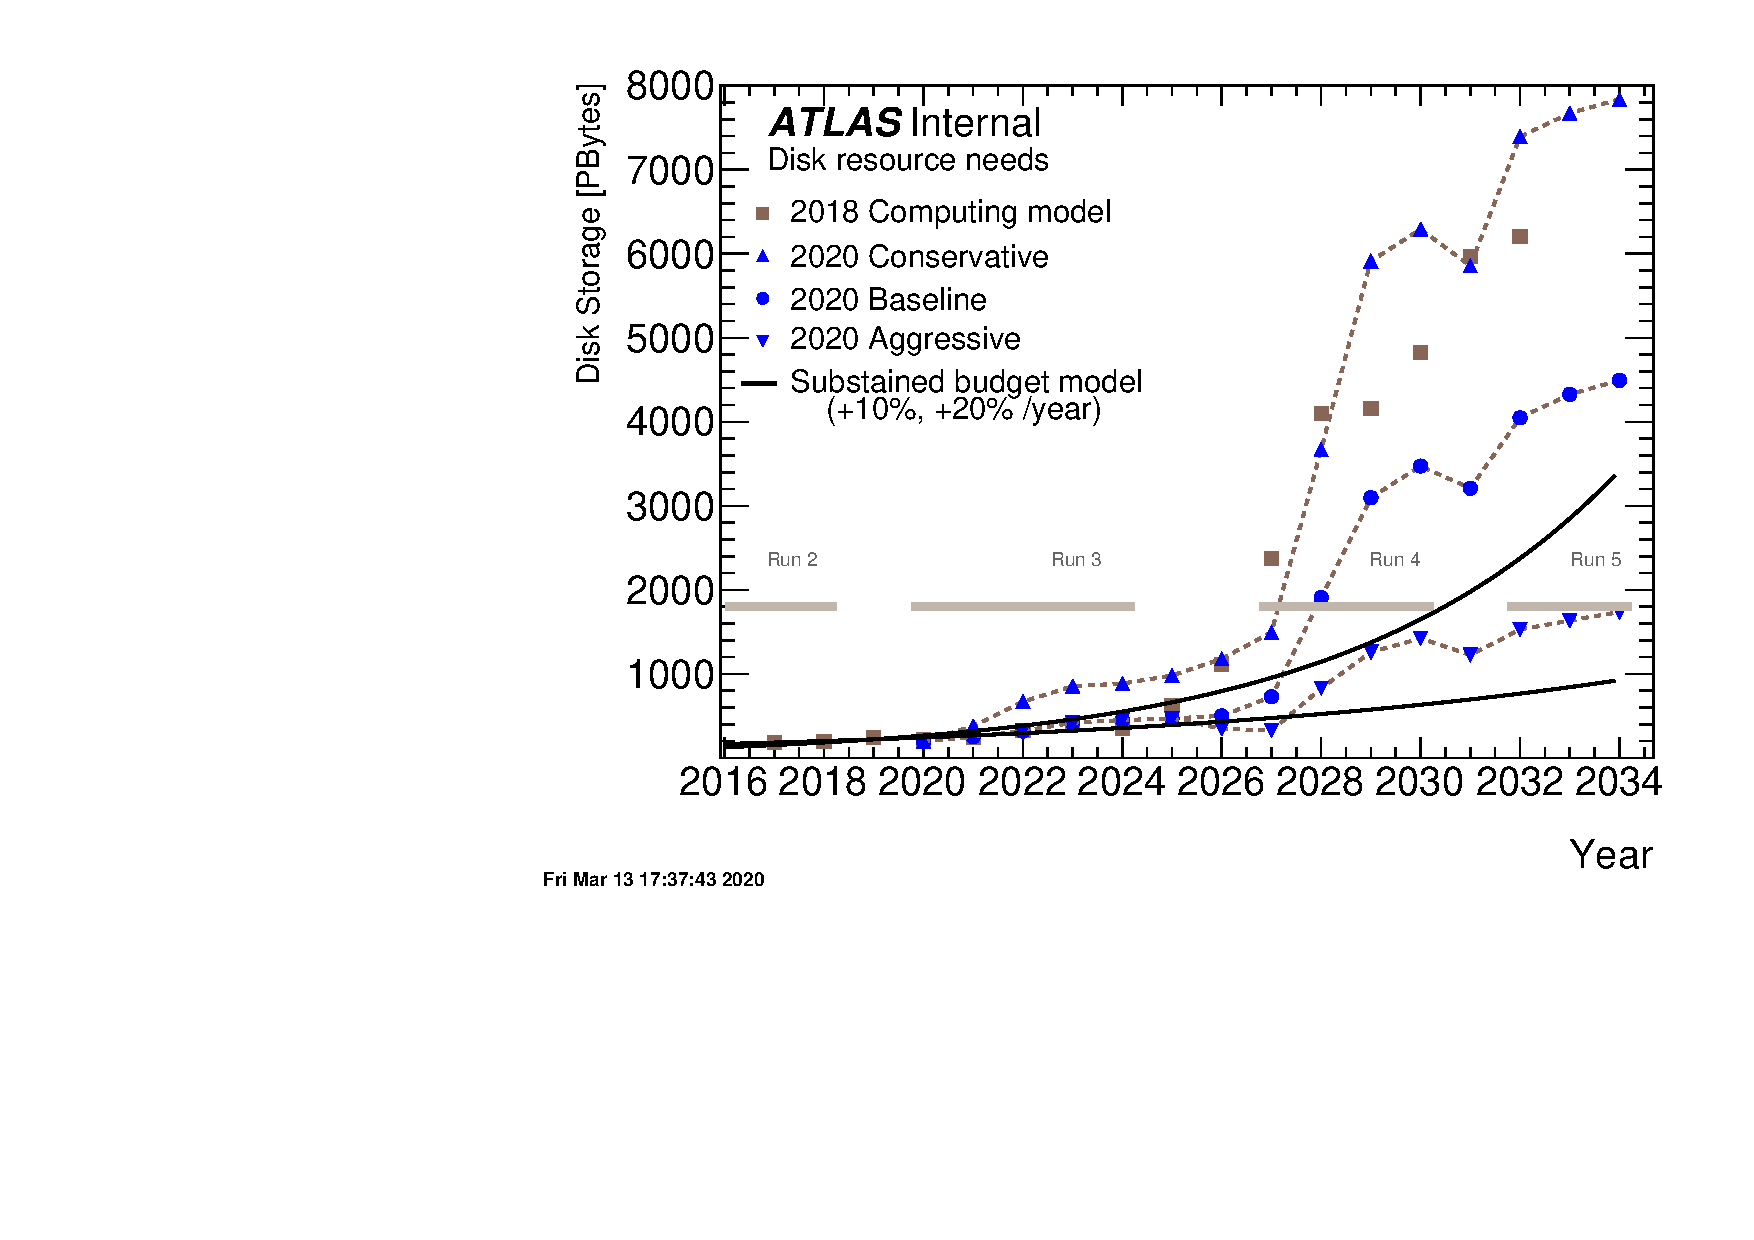
\includegraphics[width=0.80\textwidth]{figures/diskHLLHC_comparison_plot_2020_InputData_11March.pdf}
   \caption{ Estimated  total Disk resources  needed for the years 2020 to 2034.  }  
    \label{fig:disk}
\end{figure}




Here we update the plots that have been shown. We should have plots also for tape (or long-term storage) needs. 
Plots on the impact on physics performances should also be added, either here or in a different section